% !TeX root = ../Bachelorarbeit.tex
\chapter{Konzeption}
\section{Prototypenaufbau}

\begin{center}
    \center
    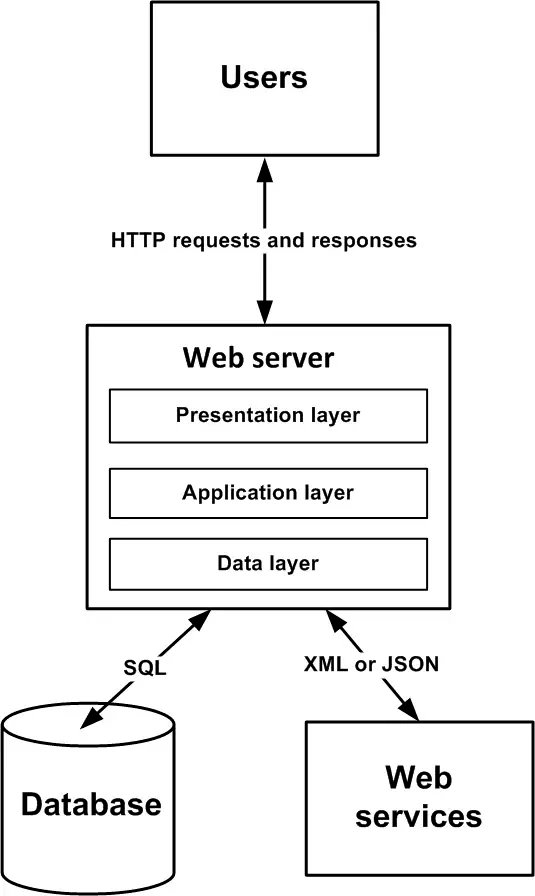
\includegraphics[width=10cm]{main-qimg-82af1fe49f85a31700d35570189a1fce.png}
\end{center} 

Das Ziel des Prototypen ist es, wie eingangs erwähnt, vorhandene Authentifizierungsverfahren abseits der klassischen UserID / Passwort Methode zu begutachten und dessen Schwächen aufzudecken. Daraus ergeben sich die typischen drei Komponenten von Drei-Tier-Client-Server Architekturen:

Ein Client, der Anfragen an die Applikation (das Backend bzw. den Server) sendet, welches die Daten dann in einer Datenbank mittels eines DBMS (Datenbankmanagementsystems) persistiert und verwaltet. Wie auch im Bild zur 3 Tier Architektur zu sehen, agiert der User auf dem Presentation Layer und stellt anfragen bzw. sendet JSON Objekte an den Server, der die entsprechenden Webservices liefert. Der Server speichert keine States, wodurch der Nutzer typischerweise mit jeder Anfrage alle benötigten Informationen liefern muss. Der Server liefert demnach lediglich die \ac{rest} Schnittstellen.

\begin{enumerate} 
\item \textbf{Client / Webseite}

Die Webseite besteht aus einer zur \ac{spa} ähnlichen Architektur, die ausschließlich Javascript und JQuery, also clientseitige Programmiersprachen nutzt. SPA's sind Webapplikationen, bei denen der Nutzer eine Seite betritt und diese nie wieder vollständig laden muss. Frameworks wie Angular, React oder VueJS basieren auf dieser Mechanik und nutzen Javascript und JQuery um die Ladezeiten einer Webseite durch Module zu reduzieren. Anstatt also die gesamte Webseite neuzuladen, laden diese Frameworks nur spezielle Bereiche der Webseite asynchron nach. In meinem Prototyp ist dies größtenteils der Fall, da neben der Hauptseite \textbf{index.html} eine weitere Seite existiert, auf die man bei erfolgreichem Login weitergeleitet wird: \textbf{secret\_panel.html}. Auch werden keine Module nachgeladen, sondern bei entsprechender Aktion nur Elemente innerhalb des DOM - Baums per id identifiziert und versteckt.

Beim Betreten von beiden Seiten der Anwendung findet eine Prüfung nach dem Session-Cookie (\textbf{user\_sid}) statt, die vom Server bei einer erfolgreichen Authentifikation im Header über 'Set-Cookie' als Response zurückkommt und vom Browser in folge dessen gesetzt wird. Der Aufruf der \textbf{index.html} Seite ist nicht möglich mit gesetztem Cookie und leitet den User auf \textbf{secret\_panel.html} weiter und umgekehrt genauso. Die Sicherung dieses Cookies auf Serverseite durch Prüfungen ist nicht Bestandteil dieser Arbeit, hier wird sich ledeglich auf den Loginprozess von Anwendungen konzentriert um dessen Schwächen und die Vorteile neuer Verfahren aufzuzeigen. Aktuell könnte ein Angreifer demnach selbst einen entsprechenden Cookie mit einem Wert setzen und das 'geheime Panel' erreichen. Bei weiter ausgereiften Webapplikationen wird bei jedem Request an den Server der Session Cookie mit einer temporären Map innerhalb des Backends abgeglichen. Befindet sich der Session Cookie nicht in dieser Map oder hat nicht genügend Rechte für diese Anfrage, erhält der Nutzer den Statuscode 401 (Unauthorized) zurück. So haben es etablierte Dienste wie 'Netflix' und 'Microsoft' bereits umgesetzt.

Aus der Forschungsfrage ergibt sich, dass die Webseite ausschießlich Javascript (oder auf Javascript basierende Programmiersprachen wie JQuery) zur Implementation der Programmlogik verwendet. Javascript selbst ist eine clientseitige Programmiersprache und gibt dem Nutzer den gesamten Code auf Webseiten preis. Demnach wurde bei der Anwendung darauf geachtet, alle clientseitigen Prüfungen, auch serverseitig zu implementieren. Zumindestens alle wichtigen Prüfungen, die sonst den Programmablauf verhindern würden oder sogar Serverabstürze zur Folge hätten. Nicht nur gibt Javascript den Code preis, über die Konsole (Unter Google Chrome und Firefox in den Entwickleroptionen des Browsers zu finden) lassen sich ganze Funktionen oder globale Variablen manipulieren. Variablen innerhalb von Funktionen können vom Angreifer nicht so leicht manipuliert werden.

Möglich ist es dennoch, den Inhalt dieser Funktion in eine andere Funktion zu schreiben, um die Variable dort auszutauschen. Um dem Nutzer nicht jede Funktion problemlos erreichbar zu machen, wurde bei der Implementation das Revealing-Module-Pattern angewendet, über die gewisse Variablen nicht im globalen Scope (window) sondern im Scope einer Funktion bleiben, die nur gewisse andere Funktionen in sich exportiert und als eine Art Schnittstelle fungiert. Auf dieses Pattern wird im Folgenden näher eingeggangen.

Das Design der Webanwendung ist kein wesentlicher Punkt dieser Arbeit und deshalb schlicht gehalten. So besteht der Prototyp aus einer einfachen Webseite, die aus dem globalen Internet erreichbar sein wird und die zwei Eingabefelder und einen Loginbutton besitzt. Die unterschiedlichen Methoden der Authentifizierung wählt man über ein Dropdownmenü über dem Login - Button. Je nach Authentifizierungsverfahren werden kleine Popup-Boxen sichtbar, die die weiteren Schritte für die Authentifikation erläutern. Die Methode kann sowohl über das Dropdownmenü als auch über einen Klick auf die Pfeile links und rechts neben dem Dropdownmenü gewählt werden, die als Pagination zwischen den verschiedenen behandelten Verfahren fungiert. Ist man am Ende der drei Methoden, springt man wieder zur ersten Methode und andersherum.

Bei der Web Authentication gibt es eine Besonderheit. Die Webseite auf die Schnittstellen des Betriebssystems zugreifen, um den Nutzer zu verifizieren. Dieser Teil kann von meinem Prototyp nicht beeinflusst werden und wird vom CTAP2 innerhalb des FIDO2 Standards definiert. Dadurch entstehen teilweise merkwürdige und aus UX (User Experience) - Sicht höchst fragwürdige Interaktionen. So fragt das Betriebssystem zunächst (bei entsprechender Möglichkeit) nach einem PIN um den Nutzer zu registrieren. Drückt man nun die Escape-Taste erscheint ein Dialog um einen Sicherheitsschlüssel (ein externes Gerät) einzurichten. Beim Login wiederrum ist dies durch eine Dropdownliste schöner gelöst worden, wo der User alle möglichen Loginmethoden auf einem Blick sieht und diese Wählen kann. Während er bei der Registration keine Chance hat dies zu tun und immer erst ein PIN - Feld angezeigt wird. Auf die einzelnen behandelten Verfahren wird in späteren Kapiteln noch genauer eingeggangen, da werden solche Schwierigkeiten aufgegriffen da dies nur eines von vielen 'Problemen' neuerer Verfahren ist: Die Abhängigkeit vom Betriebssystem.

Das Design der Website ist recht schlicht. Um sich die Designarbeit oder das Suchen von Icons und passenden Buttondesigns zu sparen wurde auf bekannte Frameworks wie Bootstrap4 und Funktionalitäten wie Flexbox gesetzt, die eine automatisches Rescaling und Positioning beinhalten. So war es nicht nötig ein Loginformular zu designen sondern vorhandene Strukturen von Bootstrap für Buttons aller Art zu nutzen.

\item \textbf{Server}

Der NodeJS - Server besteht aus einer REST Api, die keine Zustände speichert. Neben der Aufgabe des Cookie Managements und der Generierung von UUID's liefert er zudem die Schnittstelle zur Datenbank und verschiedene Funktionalitäten für die behandelten Verfahren Username \& Passwort, TOTP und Webauthn:

\begin{itemize}
 \item \textbf{/logout} - POST
 
 Löscht den Session-Cookie (und damit die Session des Nutzers) und leitet ihn auf die Loginseite \textbf{index.html} weiter.

 \item \textbf{/get\_public\_key} - GET
 
 Liest den öffentlichen Schlüssel des Servers ein und gibt diesen in einer JSON - Struktur zurück. Ist wichtig für die Username \& Passwort - Authentifizierung.
 \newpage

 \item \textbf{/password/login} - POST
 
 Nimmt einen mit dem öffentlichen Schlüssel des Servers verschlüsselten Usernamen und Passwort entgegen und entschlüsselt diese mit dem privaten Schlüssel. Im Anschluss darauf wird in der Datenbank über einen gepoolte Query (eine Anzahl an Verbindungsprozessen zur Datenbank) nach dem Nutzer gesucht. Wurde dieser gefunden, erstellt der Server einen SHA512 - Hash aus dem Passwort (aus dem Request) und dem Salt des Users (aus der Datenbank) indem die \textbf{hashString} - Methode aufgerufen wird. Diese arbeitet mit der crypto Library um den Hash zu generieren und bezieht den Pepper des Servers mit ein. Sofern die Hashes aus der Datenbank und der soeben Generierte übereinstimmen, erhält der Nutzer die Response 200 und den Text ``OK''. Gleichzeitig wird wie bei jeder anderen Authentifizierungsmethode die \textbf{createSessionCookie} - Methode aufgerufen um den Session-Cookie (eine zufällige UUID) im Header zurück an den Nutzer zu senden, sodass dieser ihn im Browser.
 
 \item \textbf{/password/create\_password\_hash} - GET
 
 Nimmt eine Zeichenkette des Nutzers entgegen und erstellt einen Password-Hash für den Nutzer, der manuell in die Datenbank persistiert werden kann. Ist als 'Quality of Service' Funktion zu verstehen, um es dem Administrator einfacher zu machen, Passwörter zu erstellen, die bei Vergleich einen gülltigen Hash ergeben.
 
 \item \textbf{/totp/check\_username} - POST
 
 Diese Methode dient lediglich der Prüfung, ob der Nutzer die TOTP Authentifikation mittels zufälligem SECRET bereits gegenüber der Webseite validiert hat. Das Datenbankfeld 'totp\_activated' wird hier geprüft, ist der Wert 1 (stehen für das boolsche 'wahr') liefert der Server den Text ``Success'' zurück, das der Client deutet um nur das Feld für den sechsstelligen OTP Code anzuzeigen. Hat das Feld allerdings den Wert 0, wird entweder (sofern noch nicht vorhanden im Feld 'totp\_secret') ein neues Secret erstellt und in der Datenbank für diesen Nutzer persistiert. Gleichzeitig für eine URL beginnend mit otp:// erstellt, um diesen zusammen mit einem Base 64 enkodierten QR Code an den Client geschickt, der dies dem User präsentiert. Es wurde sich hier bewusst dazu entschieden, diese Schritte auf Serverseite vorzunehmen. Möglich wäre es auch auf Clientseite gewesen, wäre aber mit einem Mehraufwand verbunden, welches hier verhindert werden sollte.
 \newpage
 
 \item \textbf{/totp/check\_token} - POST
 
 Nimmt den Usernamen des Nutzers und einen sechsstelligen TOTP Token entgegen. Sucht im Anschluss darauf in der Datenbank nach dem Nutzer und prüft über die Library 'otplib' ob der eingegebene TOTP - Token zum secret in der Datenbank valide ist. Dieser Schritt findet sowohl bei der Registration als auch beim Login statt. Wenn das Feld 'totp\_activated' also 0 ist, wird es bei der ersten Authentifikation auf 1 gesetzt und der Nutzer wird eingeloggt. (Session-Cookie wird gesetzt und nutzer weitergeleitet)
\end{itemize}

\item \textbf{Datenbank} (Schadensauswirkungen können ein existenziell bedrohliches Ausmaß annehmen
\end{enumerate}

Neben den vorhandenen Methoden soll die eigene Architektur aufgebaut werden, die sich an vorhandenen Authentifikationsmöglichkeiten bedient. Die UserID und das Passwortfeld sind beim ersten Aufruf der Seite zwar zu sehen, müssen allerdings nicht zwingend für jedes der Verfahren genutzt werden, so kann es zum Beispiel bei einer besitzbasierten Authentifikation bereits reichen, den Besitz (z.B einen USB - Stick, welcher einen privaten Schlüssel beherbergt) im Computer einstecken zu haben und auf den Loginbutton zu drücken. Bei der Architektur muss zwingend eine Datenbank und ein Backend zur Webseite implementiert werden um einerseits die eingegangenen Daten zu bearbeiten und andererseits in die Datenbank zu persistieren. Das Dropdownmenü zeigt die Authentifikation über biologische Merkmale (Touch ID oder Face ID) nur sofern das Gerät, auf welchem der Prototyp bedient wir, einen entsprechenden Sensor und die entsprechende Software zur Verarbeitung besitzt.

\section{Auswahl der Authentifizierungsverfahren}
Neben des altbekannten \ac{totp} Verfahrens, wird das Secure Element und die E-Mail Authentifikation betrachtet. Dabei bedienen sich diese Verfahren aller drei Möglichkeiten der Authentifikation, dem Wissen, dem Besitz und der körperlichen Merkmale. 

\section{Kriterien zur Bewertung des Prototypen}
\section{Architektur}
